% !TeX spellcheck = en_US
\documentclass[letterpaper,12pt,twoside]{report}
\usepackage{fancyhdr}
\usepackage{fullpage}
\usepackage{tikz}
\usepackage{amsmath}

\begin{document}
	\pagestyle{fancy}
	\fancyhf{}
	\fancyhead[L]{Day 15}
	\fancyhead[R]{\textit{The Calendar Project}}
	\fancyfoot[L]{Citations Involved: none}
	
	% Problem
	\paragraph{Problem}
	\begin{quote}
		\textsf{A line $p$ with positive slope
			intersects the parabola $y=x^2$
			at $A(x_1, y_1)$ and $B(x_2, y_2)$, where $y_2 = y_1 + 16$. If $A$ and $B$ are $8\sqrt{5}$ units apart, what is the equation of the line $p$ in y-intercept form?}
	\end{quote}
	
	% Graphics
	\begin{center}
		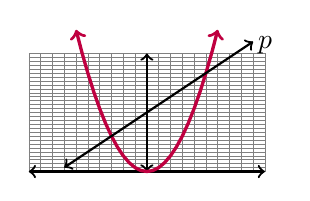
\begin{tikzpicture}[xscale=0.15,yscale=0.05]
		
		\draw[help lines] (-10,0) grid (10,30);
		\draw[<->][thick] (0,30) -- (0,0);
		\draw[<->][thick] (-10,0) -- (10,0);
		
		\draw[purple, very thick, <->, domain=-6:6] plot (\x, {\x*\x});
		\draw[black, thick, <->, domain=-7:9] plot (\x, {2*\x+15});
		\node[right] at (8.6, 32) {$p$};
		\end{tikzpicture}
	\end{center}
	
	% Reasoning
	\paragraph{Reasoning}
	\begin{quotation}
		
		Since it is given that the parabola $y=x^2$ is intersected at $A$ and $B$, these points lie on the parabola and thus fulfill the equations $y_1=x_1^2$ and $y_2=x_2^2$. Using the distance formula, the distance between $A$ and $B$ can be represented by the expression $\sqrt{(x_2-x_1)^2+(y_2-y_1)^2}$, which is given to be equal to $8\sqrt{5}$; both sides are multiplied by themselves to produce to equation $(x_2-x_1)^2+(y_2-y_1)^2=320$. Given that $y_2=y_1+16$, $y_2-y_1=16$ when both sides are subtracted by $y_1$, and $y_2-y_1$ can be substituted as $16$ in the equation derived from the Distance Formula, which can be simplified: $(x_2-x_1)^2+16^2=320=(x_2-x_1)^2+256$; after subtracting both sides by 256, $(x_2-x_1)^2=64$ and thus $x_2-x_1=\sqrt{64}=8$. The variables are then determined below:
		\begin{center}
			\begin{tabular}{l | l}
				$y_1=x_1^2$, $y_2=x_2^2$, $x_2-x_1=8$, $y_2-y_1=16$ & As derived above \\
				$x_2^2-x_1^2=16$ & Substitution \\
				$x_2=8+x_1$ & Add both sides by $x_1$ \\
				$(8+x_1)^2-x_1^2=16$ & Substitution \\
				$(64+16x_1+x_1^2)-x_1^2=16$ & Expand the squared term \\
				$64+16x_1=16$ & Simplify \\
				$16x_1=16-64=-48$ & Subtract both sides by 64 and Simplify \\
				$x_1=\dfrac{-48}{16}=-3$ & Divide both sides by 16 and Simplify \\
				$y_1=(-3)^2=9$ & Substitution and Simplify \\
				$x_2=8+(-3)=5$ & Substitution and Simplify \\
				$y_2=(5)^2=25$ & Substitution and Simplify
			\end{tabular}
		\end{center}
	
		The slope of line $p$ can be determined using the slope formula: $\frac{y_2-y_1}{x_2-x_1}=\frac{25-9}{5-(-3)}=\frac{16}{8}=2$. Given that point $A(x_1,y_1)$ lies on line $p$, the line can be represented using an equation in point-slope form: $y-y_1=m(x-x_1) \Rightarrow y-9=2(x-(-3))=2(x+3)$. Using the distributive property, $2(x+3)=2x+6$. For $y-9=2x+6$, adding 9 to both sides yields $\boxed{y=2x+15}$, the solution to this problem.
	\end{quotation}
	
\end{document}